% chap10 - Second-order systems
% Last edited:

\chapter{Second-order systems}


\section{Nested functions}

In the Section~\ref{funfiles}, we saw an example of an M-file with
more than one function:

\begin{verbatim}
function res = duck()
  error = error_func(10)
end

function res = error_func(h)
  rho = 0.3;   % density in g / cm^3
  r = 10;     % radius in cm
  res = ...
end
\end{verbatim}

Because the first function ends before the second begins, they are at
the same level of indentation. Functions like these are {\bf
parallel}, as opposed to {\bf nested}. A nested function is
defined inside another, like this:

\begin{verbatim}
function res = duck()
  error = error_func(10)

  function res = error_func(h)
    rho = 0.3;   % density in g / cm^3
    r = 10;     % radius in cm
    res = ...
  end
end
\end{verbatim}

The top-level function, {\tt duck}, is
the {\bf outer function} and {\tt error\_func} is
an {\bf inner function}.

Nesting functions is useful because the variables of the outer
function can be accessed from the inner function. This is not
possible with parallel functions.

In this example, using a nested function makes it possible to
move the parameters {\tt rho} and {\tt r} out of {\tt error\_func}.

\begin{verbatim}
function res = duck(rho)
  r = 10;
  error = error_func(10)

  function res = error_func(h)
    res = ...
  end
end
\end{verbatim}

Both {\tt rho} and {\tt r} can be accessed from {\tt error\_func}.
By making {\tt rho} an input argument, we made it easier to test
{\tt duck} with different parameter values.



\section{Newtonian motion}

Newton's second law of motion is often written like this

\[ F = ma \]

where $F$ is the net force acting on a object, $m$ is the mass
of the object, and $a$ is the resulting acceleration of the object.
In a simple case where the object is moving along a straight line,
$F$ and $a$ are scalars, but in general they are vectors.

Even more generally, if $F$ and $a$ vary in time, then they can
be thought of as functions that return vectors; that is, $F$ is
a function and the result of evaluating $F(t)$ is a vector that
describes the net force at time $t$. So a more explicit way to
write Newton's law is

\[ \forall t: \vec{F}(t) = m \vec{a}(t) \]

The arrangement of this equation suggests that if you know $m$ and $a$
you can compute force, which is true, but in most physical
simulations it is the other way around. Based on a physical
model, you know $F$ and $m$, and compute $a$.

So if you know acceleration, $a$, as a function of time, how do you
find the position of the object, $p$? Well, we know that acceleration
is the second derivative of position, so we can write a differential
equation

\[ p_{tt} = a \]

Where $a$ and $p$ are functions of time that return vectors,
and $p_{tt}$ is the second time derivative of $p$.

Because this equation includes a second derivative, it is a second-order
ODE. {\tt ode45} can't solve this equation in this form, but by
introducing a new variable, $v$, for velocity, we can rewrite it as
a system of first-order ODEs.

\begin{eqnarray*}
p_t &=& v \\
v_t &=& a
\end{eqnarray*}

The first equation says that the first derivative of $p$ is $v$; the
second says that the derivative of $v$ is $a$.


\section{Freefall}
\label{freefall}

Let's start with a simple example, an object in freefall in a vacuum
(where there's no air resistance). Near the surface of the earth, the
acceleration of gravity is $g = -9.8$ $m/s^2$, where the minus sign
indicates that gravity pulls down.

If the object falls straight down (in the same direction as gravity),
we can describe its position with a scalar value, altitude. So
this will be a one-dimensional problem, at least for now.

Here is a rate function we can use with {\tt ode45} to solve
this problem:

\begin{verbatim}
function res = freefall(t, X)
  p = X(1);   % the first element is position
  v = X(2);   % the second element is velocity

  dpdt = v;             
  dvdt = acceleration(t, p, v);

  res = [dpdt; dvdt];  % pack the results in a column vector
end

function res = acceleration(t, p, v)
  g = -9.8;   % acceleration of gravity in m/s^2
  res = g;
end
\end{verbatim}

The first function is the rate function. It gets {\tt t} and
{\tt X} as input variables, where the elements of {\tt X} are understood
to be position and velocity. The return value from {\tt freefall}
is a (column) vector that contains the derivatives of position
and velocity, which are velocity and acceleration, respectively. 

Computing $p_t$ is easy because we are given velocity
as an element of {\tt X}. The only thing we have to compute is
acceleration, which is what the second function does.

{\tt acceleration} computes acceleration as a function of time,
position and velocity. In this example, the net acceleration is
a constant, so we don't really have to include all this information
yet, but we will soon.

Here's how to run {\tt ode45} with this rate function:

\begin{verbatim}
octave:1> ode45(@freefall, [0, 30], [4000, 0])
\end{verbatim}
 
As always, the first argument is the function handle, the second
is the time interval (30 seconds) and the third is the initial
condition: in this case, the initial altitude is 4000 meters and
the initial velocity is 0. So you can think of the ``object'' a
a skydiver jumping out of an airplane at about 12,000 feet.

Here's what the result looks like:

\beforefig \centerline{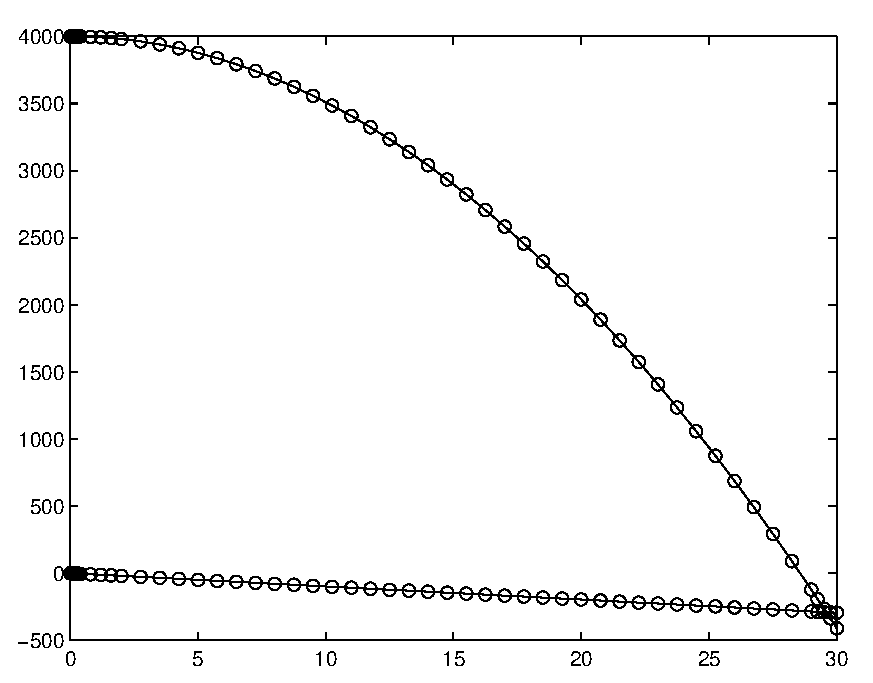
\includegraphics[height=2in]{figs/freefall.eps}}

The bottom line shows velocity starting at zero and dropping
linearly. The top line shows position starting at 4000 m and
dropping parabolically (but remember that this parabola
is a function of time, not a ballistic trajectory).

Notice that {\tt ode45} doesn't know where the ground is, so the
skydiver keeps going through zero into negative altitude. We will
address this issue later.


\section{Air resistance}

To make this simulation more realistic, we can add air resistance.
For large objects moving quickly through air, the force due to air
resistance, called ``drag,'' is proportional to $v^2$:

\[ F_{drag} = c v^2 \]

Where $c$ is a drag constant that depends on the density of
air, the cross-sectional area of the object and
the surface properties of the object. For purposes of this
problem, let's say that $c = 0.2$.

To convert from force to acceleration, we have to know mass, so let's
say that the skydiver (with equipment) weighs 75 kg.

Here's a version of {\tt acceleration} that takes air resistance
into account (you don't have to make any changes in {\tt freefall}:

\begin{verbatim}
function res = acceleration(t, p, v)
  a_grav = -9.8;       % acceleration of gravity in m/s^2
  c = 0.2;          % drag constant
  m = 75;           % mass in kg
  f_drag = c * v^2;      % drag force in N
  a_drag = f_drag / m;    % drag acceleration in m/s^2
  res = a_grav + a_drag;   % total acceleration
end
\end{verbatim}

The sign of the drag force (and acceleration) is positive as
long as the object is falling, the direction of the drag force is
up.
The net
acceleration is the sum of gravity and drag. Be careful when you
are working with forces and accelerations; make sure you only add
forces to forces or accelerations to accelerations. In my code,
I use comments to remind myself what units the values are in.
That helps me avoid nonsense like adding forces to accelerations.

Here's what the result looks like with air resistance:

\beforefig \centerline{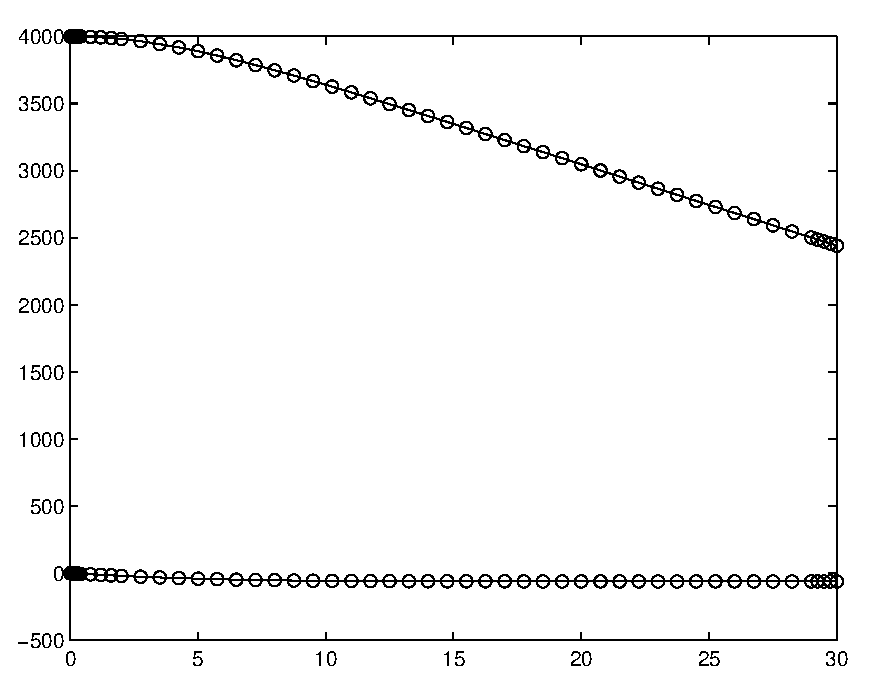
\includegraphics[height=2in]{figs/freefall2.eps}}

Big difference! With air resistance, velocity increases until
the drag acceleration equals $g$; after that, velocity is a constant,
known as ``terminal velocity,'' and position decreases linearly
(and much more slowly than it would in a vacuum). To examine
the results more closely, we can assign them to variables


\begin{verbatim}
octave:1> [T, M] = ode45(@freefall, [0, 30], [4000, 0]);
\end{verbatim}

And then read the terminal position and velocity:

\begin{verbatim}
octave:1> M(end,1)

ans = 2.4412e+03     % altitude in meters

octave:1> M(end,2)

ans = -60.6143      % velocity in m/s
\end{verbatim}

\begin{ex}
Increase the mass of the skydiver, and confirm that
terminal velocity increases. This relationship is the source of the
intuition that heavy objects fall faster; in air, they do!
\end{ex}


\section{Parachute!}

In the previous section, we saw that the terminal velocity of a $75
kg$ skydiver is about 60 $m/s$, which is about 130 mph. If you hit
the ground at that speed, you would almost certainly be killed.
That's where parachutes come in.

\begin{ex}
Modify {\tt acceleration} so that after 30 seconds of
free-fall the skydiver deploys a parachute, which (almost) instantly
increases the drag constant to 2.7.

What is the terminal velocity now? How long (after deployment) does
it take to reach the ground?
\end{ex}


\section{Two dimensions}
\label{projectile}

So far we have used {\tt ode45} for a system of first-order
equations and for a single second-order equation. The next logical
step is a system of second-order equations, and the next logical example
is a projectile. A ``projectile'' is an object propelled
through space, usually toward, 
and often to the detriment of,
a target.

If a projectile stays in a plane, we can think of the system as
two-dimensional, with $x$ representing the horizontal distance
traveled and $y$ representing the height or altitude. So now
instead of a skydiver, think of a circus performer being fired
out of a cannon.

According to the
Wikipedia\footnote{\url{http://en.wikipedia.org/wiki/Human_cannonball}},
the record distance for a human cannonball is 56.5 meters (almost 186
feet).

Here is a general framework for computing the trajectory of a projectile
in two dimensions using {\tt ode45}:

\begin{verbatim}
function res = projectile(t, W)
  P = W(1:2);
  V = W(3:4);

  dPdt = V;             
  dVdt = acceleration(t, P, V);

  res = [dPdt; dVdt];
end

function res = acceleration(t, P, V)
  g = -9.8;       % acceleration of gravity in m/s^2
  res = [0; g];
end
\end{verbatim}

The second argument of the rate function is a vector, {\tt W}, with
four elements. The first two are assigned to {\tt P}, which
represents position; the last two are assigned to {\tt V}, which
represents velocity.
{\tt P} and {\tt V} are vectors with
elements for the $x$ and $y$ components.

The result from
{\tt acceleration} is also a vector; ignoring air resistance
(for now), the acceleration in the $x$ direction is 0; in
the $y$ direction it's $g$.
Other than that, this code is similar to what we saw in
Section~\ref{freefall}.

If we launch the human projectile from an initial height of
3 meters, with velocities 40 m/s and 30 m/s in the $x$ and $y$
directions, the {\tt ode45} call looks like
this:

\begin{verbatim}
ode45(@projectile, [0,10], [0, 3, 40, 30]);
\end{verbatim}

And the result looks like this:

\beforefig \centerline{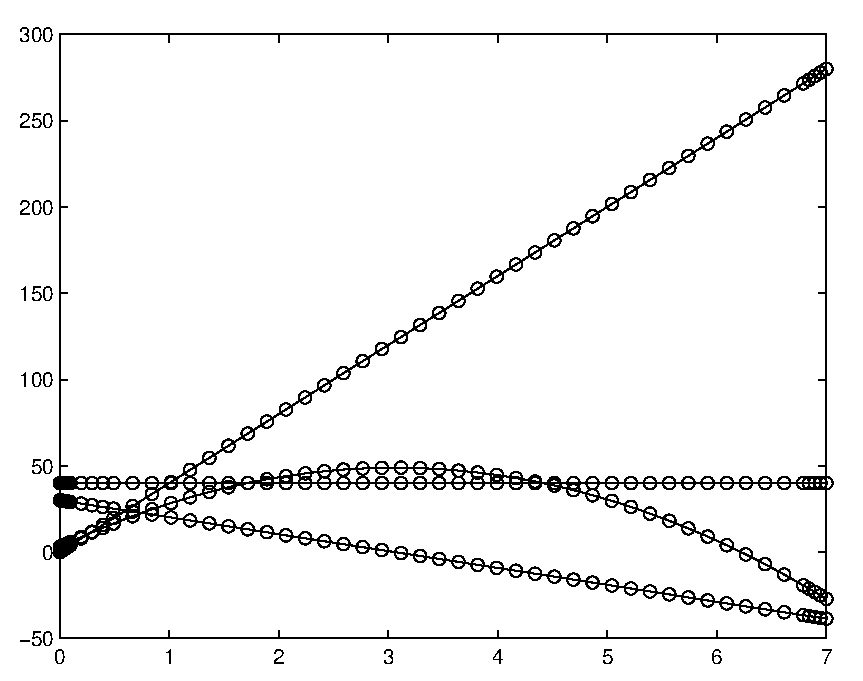
\includegraphics[height=2in]{figs/proj1.eps}}

You might have to think a little to figure out which line is
which. It looks like the flight time is about 6 seconds.

\begin{ex}
Extract the $x$ and $y$ components of
position, plot the trajectory of the projectile, and estimate the
distance traveled.
\end{ex}

\begin{ex}
Add air resistance to this simulation. In
the skydiver scenario, we estimated that the drag constant was
$0.2$, but that was based on the assumption that the skydiver is
falling flat. A human cannonball, flying head-first, probably
has a drag constant closer to $0.1$. What initial velocity
is needed to achieve the record flight distance of 65.6 meters?
Hint: what is the optimal launch angle?
\end{ex}


\section{What could go wrong?}

What could go wrong? Well, {\tt vertcat} for one. To explain
what that means, I'll start with {\bf catenation}, which is
the operation of joining two matrices into a larger matrix.
``Vertical catenation'' joins the matrices by stacking them on
top of each other; ``horizontal catenation'' lays them
side by side.

Here's an example of horizontal catenation with row vectors:

\begin{verbatim}
octave:1> x = 1:3

x = 1   2   3

octave:1> y = 4:5

y = 4   5

octave:1> z = [x, y]

z = 1   2   3   4   5
\end{verbatim}

Inside brackets, the comma operator performs horizontal catenation.
The vertical catenation operator is the semi-colon. Here is an
example with matrices:

\begin{verbatim}
octave:1> X = zeros(2,3)

X = 0   0   0
   0   0   0

octave:1> Y = ones(2,3)

Y = 1   1   1
   1   1   1

octave:1> Z = [X; Y]

Z = 0   0   0
   0   0   0
   1   1   1
   1   1   1
\end{verbatim}

These operations only work if the matrices are the same size along
the dimension where they are glued together. If not, you get:

\begin{verbatim}
octave:1> a = 1:3

a = 1   2   3

octave:1> b = a'

b = 1
   2
   3

octave:1> c = [a, b]
??? Error using ==> horzcat
All matrices on a row in the bracketed expression must have the 
 same number of rows.

octave:1> c = [a; b]
??? Error using ==> vertcat
All rows in the bracketed expression must have the same 
number of columns.
\end{verbatim}

In this example, {\tt a} is a row vector and {\tt b} is a column
vector, so they can't be catenated in either direction.

Reading the error messages, you probably guessed that {\tt horzcat}
is the function that performs horizontal catenation, and likewise
with {\tt vertcat} and vertical catenation.

These operations are relevant to {\tt projectile} because of the
last line, which packs {\tt dPdt} and {\tt dVdt} into the
output variable:

\begin{verbatim}
function res = projectile(t, W)
  P = W(1:2);
  V = W(3:4);

  dPdt = V;             
  dVdt = acceleration(t, P, V);

  res = [dPdt; dVdt];
end
\end{verbatim}

As long as both {\tt dPdt} and {\tt dVdt} are column vectors,
the semi-colon performs vertical catenation, and the result is
a column vector with four elements. But if either of them is a
row vector, that's trouble.

{\tt ode45} expects the result from {\tt projectile} to be a
column vector, so if you are working with {\tt ode45}, it is
probably a good idea to make {\em everything} a column vector.

In general, if you run into problems with {\tt horzcat} and {\tt
vertcat}, use {\tt size} to display the dimensions of the operands,
and make sure you are clear on which way your vectors go.


\section{Glossary}

\begin{description}

\item[parallel functions:] Two or more functions defined side-by-side,
so that one ends before the next begins.

\item[nested function:] A function defined inside another function.

\item[outer function:] A function that contains another function
definition.

\item[inner function:] A function defined inside another function
definition. The inner function can access the variables of the
outer function.

\item[catenation:] The operation of joining two matrices end-to-end to
form a new matrix.


\end{description}

\section{Exercises}

\begin{ex}
\label{baseball}

The flight of a baseball is governed by three forces: gravity,
drag due to air resistance, and Magnus force due to spin. If
we ignore wind and Magnus force, the path of the baseball stays
in a plane, so we can model it as a projectile in two
dimensions.

A simple model of the drag of a baseball is:
%
\[ F_d = -\frac{1}{2} ~ \rho ~ v^2 ~ A ~ C_d ~ \hat{V}  \]
%
where $F_d$ is a vector that represents the force on the baseball due
to drag, $C_d$ is the drag coefficient (0.3 is a reasonable choice),
$\rho$ is the density of air (1.3 kg/m$^3$ at sea level), $A$ is the
cross sectional area of the baseball (0.0042 m$^2$), $v$ is the
magnitude of the velocity vector, and $\hat{V}$ is a unit vector in
the direction of the velocity vector. The mass of the baseball is
$0.145$ kg.

For more information about drag, see
\url{http://en.wikipedia.org/wiki/Drag_(physics)}.

\begin{itemize}

\item Write a function that takes the initial velocity of the baseball
and the launch angle as input variables, uses {\tt ode45} to compute
the trajectory, and returns the range (horizontal distance in flight)
as an output variable.

\item Write a function that takes the initial velocity of the baseball
as an input variable, computes the launch angle that maximizes
the range, and returns the optimal angle and range as output variables.
How does the optimal angle vary with initial velocity?

\item When the Red Sox won the World Series in 2007, they played the
Colorado Rockies at their home field in Denver, Colorado. Find an
estimate of the density of air in the Mile High City. What effect
does this have on drag? Make a prediction about what effect this will
have on the optimal launch angle, and then use your simulation to test
your prediction.

\item The Green Monster in Fenway Park is about 12 m high and about 97
m from home plate along the left field line. What is the minimum
speed a ball must leave the bat in order to clear the monster
(assuming it goes off at the optimal angle)? Do you think it is
possible for a person to stand on home plate and throw a
ball over the Green Monster?

\item The actual drag on a baseball is more complicated than what is
captured by our simple model. In particular, the drag coefficient
varies with velocity. You can get some of the details from {\em The
Physics of Baseball}\footnote{Robert K. Adair, Harper Paperbacks, 3rd
Edition, 2002.}; you also might find information on the web.
Either way, specify a more realistic model of drag and modify your
program to implement it. How big is the effect on your computed
ranges? How big is the effect on the optimal angles?

\end{itemize}

\end{ex}

